\documentclass[11pt]{beamer}
\usepackage[utf8]{inputenc}
\usepackage[T1]{fontenc}
%\usepackage{natbib}
\usetheme{Pittsburgh}
\usepackage{verbatim} 
\usepackage[english]{babel}
\usepackage{epstopdf}
\usepackage{minted}
\usepackage{multicol}
%\titlegraphic{%\vspace*{1cm}
%	\includegraphics[width=2.5cm]{logo_udelar}
	%\hspace*{1cm}~%
%		\includegraphics[width=3.5cm]{logo_FCEA.png}
%}

\usepackage{color}

\definecolor{mygreen}{rgb}{0,0.6,0}
\definecolor{mygray}{rgb}{0.5,0.5,0.5}
\definecolor{mymauve}{rgb}{0.58,0,0.82}
\definecolor{mygray2}{rgb}{0.95,0.95,0.95}

\setbeamertemplate{navigation symbols}{}
\setbeamertemplate{footline}[frame number]
\AtBeginSection{ 
	\begin{frame}
		\frametitle{Index}
			\tableofcontents[currentsection]
	\end{frame}
}
\begin{document}
	\title{Modelos dinámicos y computacionales en Economía}
	\subtitle{Modelo de Oferta y Demanda Dinámica \\ (Modelo de la telaraña)}
	%\logo{}
	\institute{Licenciatura en Economía, FCEA, UDELAR}
	\date{7 de septiembre de 2023}
	%\subject{}
	%\setbeamercovered{transparent}
	%\setbeamertemplate{navigation symbols}{}
	\frame[plain]{\maketitle}
%\setbeamertemplate{background}{\includegraphics[width=2 cm]{logo_FCEA.png}}

\begin{frame}
\frametitle{Contenido de la clase:}
\begin{itemize}
	\item Repaso del modelo
	\begin{enumerate}
	\item Modelo original 
	\item Modelo con expectativas adaptativas
\end{enumerate}		
	\item Otras extensiones
	\begin{enumerate}
		\item Modelo con inventario 
	\end{enumerate}	
\item Solución numérica en R
	\begin{enumerate}
	\item ¿Cómo escribimos un modelo en R?
	\item Modelo original
	\item Extensiones
%	\item Funciones en R
\end{enumerate}	
\end{itemize}
\end{frame}


\begin{frame}{R: repaso de la clase pasada}
    Notar las siguientes sucesiones, a qué distribuciones pertenecen?
    \begin{figure}
        \centering
        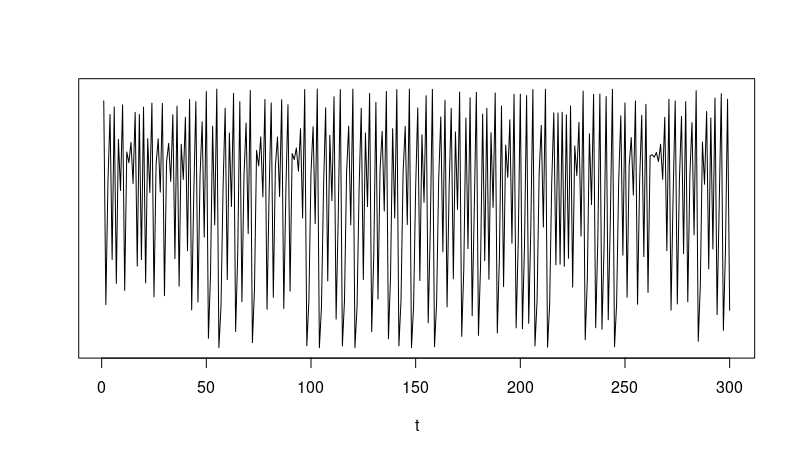
\includegraphics[width=0.32\linewidth]{plots01/Rplot01.png}
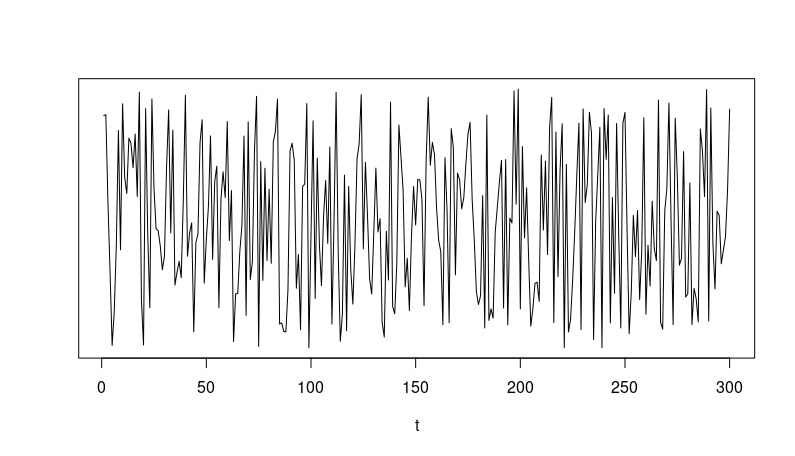
\includegraphics[width=0.32\linewidth]{plots01/Rplot02.png}
        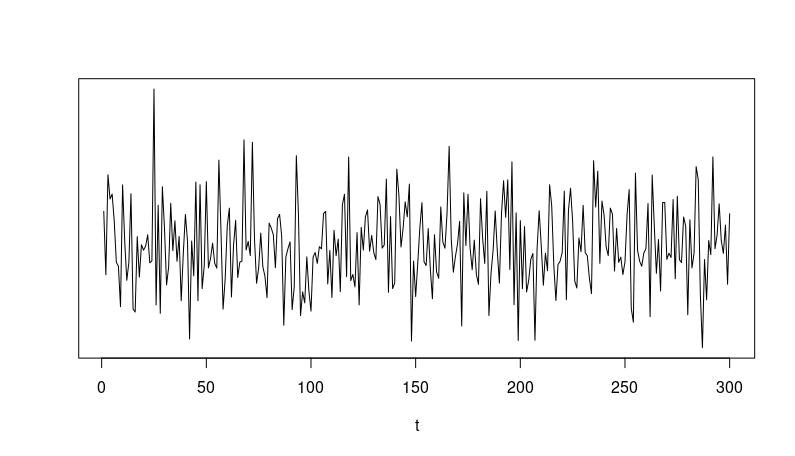
\includegraphics[width=0.32\linewidth]{plots01/Rplot03.png}
        \label{fig:my_label}
    \end{figure}
\pause
Respuesta:
        \begin{figure}
        \centering
        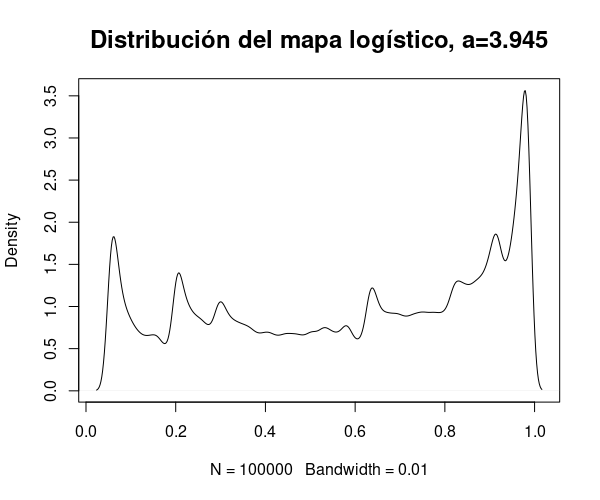
\includegraphics[width=0.32\linewidth]{plots01/Rplot04.png}
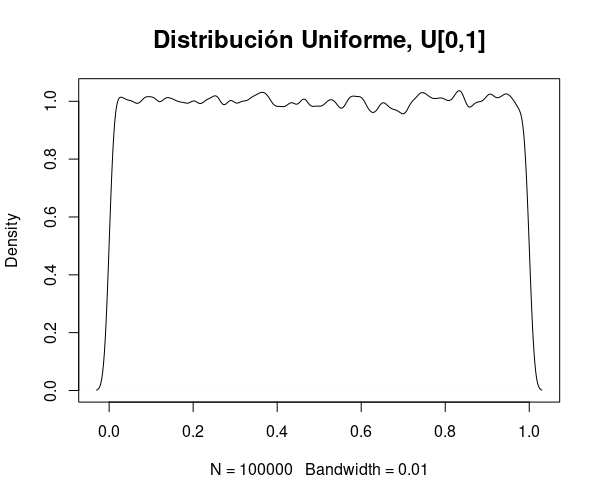
\includegraphics[width=0.32\linewidth]{plots01/Rplot05.png}
        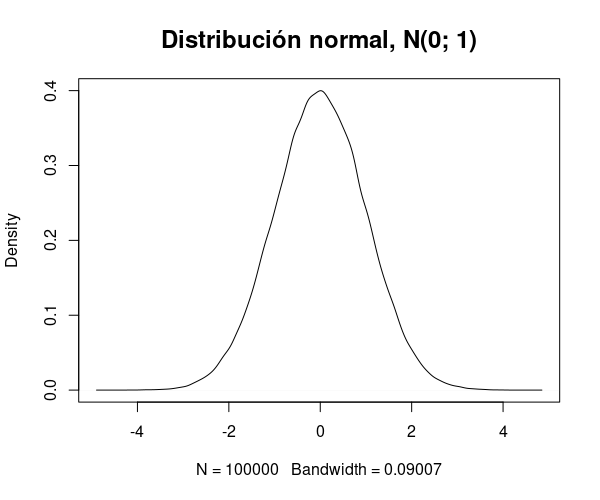
\includegraphics[width=0.32\linewidth]{plots01/Rplot06.png}
        \label{fig:my_label}
    \end{figure}
\end{frame}


\begin{frame}[fragile]{Gráficos: código de R}
\begin{minted}[bgcolor=mygray2,fontsize=\tiny]{r}        
a=3.945 ### único parámetro
q=seq(0,1,0.001)
logist=q
for (i in 1:length(q)) {
  logist[i]=a*q[i]*(1-q[i])  
}

result=vector("numeric",100000)
result[1]=0.6    
for (i in 2:length(result)){
  result[i]=a*result[i-1]*(1-result[i-1])
}

plot(result[201:500],type="l",yaxt="n",ylab="",xlab="t")
plot(runif(300),type="l",yaxt="n",ylab="",xlab="t")
plot(rnorm(300),type="l",yaxt="n",ylab="",xlab="t")



plot(density(result,bw=0.01),main="Distribución del mapa logístico, a=3.945",cex.main=1.5)
plot(density(runif(100000),bw=0.01),main="Distribución Uniforme, U[0,1]",cex.main=1.5)
plot(density(rnorm(100000)),main="Distribución normal, N(0; 1)",cex.main=1.5)
    \end{minted}
\end{frame}

\begin{frame}
\frametitle{Cobweb model: introducción}
\begin{itemize}
	\item Este modelo muestra que los precios pueden estar sujetos a fluctuaciones periódicas.
	\item Importancia del tiempo discreto.
	\item Para algunos valores de los parámetros, se alcanza el equilibrio.
	\item El comportamiento dinámico de los agentes \underline{no siempre} converge al equilibrio.
\end{itemize}
\end{frame}

\begin{frame}
\frametitle{Cobweb model: modelo original}
\framesubtitle{Presentación del modelo}
\begin{multicols}{2}
\underline{Ecuaciones:}
\begin{enumerate}
	\item $D_t=\alpha-\beta p_t$
	\item $S_t=-\gamma+\delta p_{t-1}$
	\item $D_t=S_t$ (condición de equilibrio)
\end{enumerate}
%\vspace{1.5cm}
\underline{Variables:}
\begin{itemize}
	\item D: cantidad demandada
	\item S: cantidad ofrecida
	\item p: precio
\end{itemize}
\vspace{1cm}
\underline{Parámetros: }
\begin{itemize}
	\item $\alpha, \beta$ (parámetros demanda)
	\item $\gamma, \delta$: (parámetros oferta)
\end{itemize}
\underline{Dinámica:}
\begin{equation}
p_{t+1}=-\dfrac{\delta}{\beta}p_t+\dfrac{\alpha+\gamma}{\beta}
\end{equation}	
\end{multicols}
\end{frame}

\begin{frame}
\frametitle{Cobweb model: modelo original}
\framesubtitle{Solución del modelo}	
Solución particular:
\begin{equation}\label{solpart1}
p^{*}=\dfrac{\alpha+\gamma}{\beta+\delta}
\end{equation}
Solución general:
\begin{equation}
p_t=\left( p_1-\dfrac{\alpha+\gamma}{\beta+\delta}\right) \left(-\dfrac{\delta}{\beta} \right)^{t-1}+
\dfrac{\alpha+\gamma}{\beta+\delta} 
\end{equation}
Importante:
\begin{itemize}
\scriptsize	\item La ecuación \ref{solpart1} refleja el equilibrio intertemporal del modelo.
	\item $\left( p_1-\dfrac{\alpha+\gamma}{\beta+\delta}\right)$ nos muestra si comenzamos por encima o por debajo del precio de equilibrio y la distancia a él.
	\item La expresión $\left|\dfrac{\delta}{\beta} \right|$ es importante para conocer la estabilidad del modelo: atractor si es < 1, repulsor si es > 1, oscilatorio (puntos períodicos de período 2) si es igual a 1.
\end{itemize}
\end{frame}

\begin{frame}
	\frametitle{Cobweb model: modelo con expectativas adaptativas}
	\framesubtitle{Presentación del modelo}
	\begin{multicols}{2}
		\underline{Ecuaciones:}
		\begin{enumerate}
			\item $D_t=\alpha-\beta p_t$
			\item $S_t=-\gamma+\delta p^{e}_{t}$
			\item $p^{e}_{t}=\lambda p_{t-1}+(1-\lambda) p^{e}_{t-1}$
			\item $D_t=S_t$ (condición de equilibrio)
		\end{enumerate}
		%\vspace{1.5cm}
		\underline{Variables:}
		\begin{itemize}
			\item D: cantidad demandada
			\item S: cantidad ofrecida
			\item p: precio
			\item $p^{e}$: precio esperado
		\end{itemize}
		\vspace{1cm}
		\underline{Parámetros: }
		\begin{itemize}
			\item $\alpha, \beta$ (parámetros demanda)
			\item $\gamma, \delta$ (parámetros oferta)
			\item $\lambda$: parámetro expectativas, $\lambda \in [0,1]$
		\end{itemize}
		\underline{Dinámica:}
		\begin{equation}
\small		p_{t+1}=\left[ \dfrac{\beta-\lambda(\beta+\delta)}{\beta}\right] p_t+\lambda\left( \dfrac{\alpha+\gamma}{\beta}\right)
		\end{equation}	
	\end{multicols}
\end{frame}

\begin{frame}
	\frametitle{Cobweb model: modelo con expectativas adaptativas}
	\framesubtitle{Solución del modelo}	
	Solución particular:
	\begin{equation}\label{solpart2}
	p^{*}=\dfrac{\alpha+\gamma}{\beta+\delta}
	\end{equation}
	Solución general:
	\begin{equation}
	p_t=\left( p_1-\dfrac{\alpha+\gamma}{\beta+\delta}\right) \left[ \dfrac{\beta-\lambda(\beta+\delta)}{\beta}\right]^{t-1}+
	\dfrac{\alpha+\gamma}{\beta+\delta} 
	\end{equation}
	Importante:
	\begin{itemize}
		\scriptsize	\item La ecuación \ref{solpart2} refleja el equilibrio intertemporal del modelo.
		\item $\left( p_1-\dfrac{\alpha+\gamma}{\beta+\delta}\right)$ nos muestra si comenzamos por encima o por debajo del precio de equilibrio y la distancia a él.
		\item La expresión $\left[ \dfrac{\beta-\lambda(\beta+\delta)}{\beta}\right]$ es importante para conocer la estabilidad del modelo.
	\end{itemize}
\end{frame}

\begin{frame}
	\frametitle{Cobweb model: modelo con inventario}
\framesubtitle{Introducción}	
	\begin{itemize}
		\item En este caso, levantamos el supuesto que $D_t=S_t$, $\forall t$.
		\item Como la oferta reacciona a las variaciones de precios, los productores guardan un inventario para hacer frente a imprevistos.
	\end{itemize}
\end{frame}

\begin{frame}
\frametitle{Cobweb model: modelo con inventario}
\framesubtitle{Presentación del modelo}
\begin{multicols}{2}
\underline{Ecuaciones:}
\begin{enumerate}
\item $D_t=\alpha-\beta p_t$
\item $S_t=-\gamma+\delta p_{t}$
\item $p_{t+1}=p_{t}-\sigma(S_t-D_t)$ \end{enumerate}
		%\vspace{1.5cm}
\underline{Variables:}
\begin{itemize}
\item D: cantidad demandada
\item S: cantidad ofrecida
\item p: precio
\end{itemize}
\vspace{1cm}
\underline{Parámetros: }
\begin{itemize}
\item $\alpha, \beta$ (parámetros demanda)
\item $\gamma, \delta$: (parámetros oferta)
\item $\sigma$: parámetro de ajuste de precios
\end{itemize}	
\end{multicols}
\end{frame}


\begin{frame}
\frametitle{Cobweb model: modelo con inventario}
\framesubtitle{Dinámica del modelo}
\underline{Pasos a seguir:}
\begin{itemize}
	\item sustituimos $S_t$ y $D_t$ en la tercera ecuación para que dependa sólo del precio y los parámetros.
\end{itemize}
\begin{equation}
p_{t+1}=[1-\sigma(\beta+\delta)]p_t+\sigma(\alpha+\gamma)
\end{equation}
\begin{enumerate}
	\item ¿Solución particular?
	\item ¿Solución general?
\end{enumerate}
\end{frame}

\begin{frame}
	\frametitle{Cobweb model: modelo con inventario}
	\framesubtitle{Solución particular y general del modelo}
	\begin{enumerate}
		\item Solución particular: 	\begin{equation}\label{solpart3}
		p^{*}=\dfrac{\alpha+\gamma}{\beta+\delta}
		\end{equation}
		\item Solución general:
	\begin{equation}
p_t=\left( p_1-\dfrac{\alpha+\gamma}{\beta+\delta}\right) [1-\sigma(\beta+\delta)]^{t-1}+
\dfrac{\alpha+\gamma}{\beta+\delta} 
\end{equation}

	\end{enumerate}
Importante:
\begin{itemize}
	\scriptsize	\item La ecuación \ref{solpart3} refleja (el mismo) el equilibrio intertemporal del modelo.
	\item $\left( p_1-\dfrac{\alpha+\gamma}{\beta+\delta}\right)$ nos muestra (nuevamente) si comenzamos por encima o por debajo del precio de equilibrio y la distancia a él.
	\item Estabilidad? Ver valores de $\sigma$ para los cuales la solución es estable.\\
	\onslide<2->{\textcolor{blue}{Solución: $0<\sigma<\dfrac{2}{\beta+\delta}$}}
\end{itemize}
\end{frame}

\begin{frame}
\frametitle{Escribir un modelo en R}
\framesubtitle{¿Qué datos necesitamos?}
Para escribir un modelo, necesitamos conocer:
\begin{itemize}
	\item Parámetros del modelo.
	\item Variables del modelo.
	\item Manera en que se relacionan los parámetros y las variables (ecuaciones).
	\item Valores iniciales de las variables.
\end{itemize}
\end{frame}

\begin{frame}[fragile]
	\frametitle{Escribir un modelo en R}
	\framesubtitle{Ejemplo 1: modelo Cobweb}
\begin{itemize}
	\item Dar valores a los parámetros:
	\begin{itemize}
		\item $\beta=10$; \hspace{0.55cm} $\delta=5$;
		\item $\alpha=1000$; $-\gamma=250$.
	\end{itemize}
 \begin{minted}[bgcolor=mygray2,fontsize=\tiny]{r} 
library('rootSolve')
library('pracma')
library('R.matlab')
# parámetros
a = 10
b = 5
# variables exógenas
Qd_bar = 1000 # independent / autonomous quantity demanded
Qs_bar = 250 # independent / autonomous quantity offered     
 \end{minted}
	\item Generar las variables relevantes para la dinámica (p, S, D).
 \begin{minted}[bgcolor=mygray2,fontsize=\tiny]{r} 
t = 1
P = vector("numeric",2)
Qs = vector("numeric",2)
Qd = vector("numeric",2)
\end{minted}
 \item Establecer una condición inicial para p: $p_{(t=1)}=25$
 \begin{minted}[bgcolor=mygray2,fontsize=\tiny]{r} 
P[t] = 25 # initial price
\end{minted}
\end{itemize}
\end{frame}


\begin{frame}[fragile]
	\frametitle{Escribir un modelo en R}
	\framesubtitle{Ejemplo 1: modelo Cobweb}
\begin{itemize}
\item Escribir la estructura de control para generar la dinámica del sistema:
	\begin{itemize}
		\item utilizamos la ecuación de movimiento del sistema.
		\item por 50 iteraciones (utilizar un $for$ o un $while$)
		\item Para los valores iniciales, ¿qué podemos decir de la estabilidad del modelo? \onslide<2->{Probar con:
			\begin{itemize}
				\item $\beta=\delta=10$
				\item $\beta=10$, $\delta=10.5$
			\end{itemize}}
	\end{itemize}
\end{itemize}
\begin{minted}[bgcolor=mygray2,fontsize=\tiny]{r}
t = 2
Qs[t] = Qs_bar + b * P[t - 1]
Qd[t] = Qd_bar - a * P[t - 1]
P [t] = -b/a* P[t - 1]+ ( Qd_bar-Qs_bar ) / a ;

# máximo número de periodos y tolerancia
tmax = 50
tol = 0.00001 

while ( t < tmax & abs ( P[t] - P[t-1] ) > tol * P [t]) {
  t = t + 1;
  Qs[t] = Qs_bar+b*P[t - 1] ;
  P [t] = -b/a*P[t - 1 ]+ ( Qd_bar-Qs_bar ) / a 
  Qd[t] = Qd_bar - a * P[t-1]
  
  fprintf ( " %d \t %5.2f \t %5.2f \n " , t-1, Qs[t] ,P[t] )
}
\end{minted}
\end{frame}

\begin{frame}    
	\frametitle{Escribir un modelo en R}
	\framesubtitle{Ejemplo 1: modelo Cobweb}
\begin{figure}
        \centering
        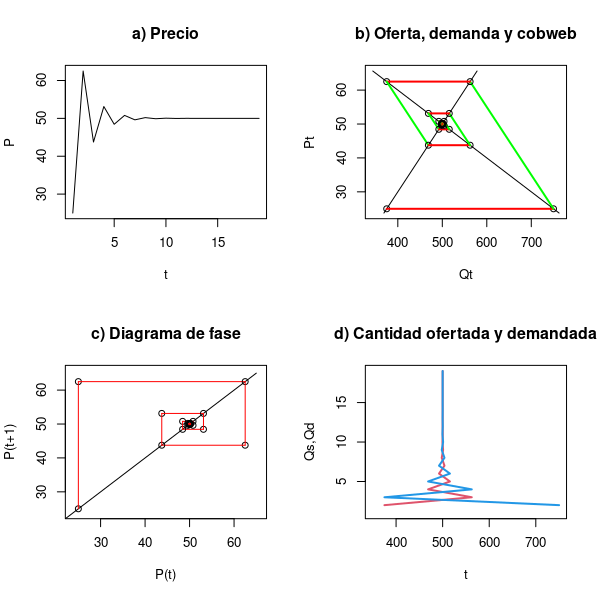
\includegraphics[width=0.7\linewidth]{plots01/Rplot07.png}
    \end{figure}
\end{frame}

\begin{frame}[fragile]
	\frametitle{Escribir un modelo en R}
	\framesubtitle{Ejemplo 1: modelo Cobweb}
\begin{minted}[bgcolor=mygray2,fontsize=\tiny]{r}
op <- par(mfrow = c(2, 2))
### plot 1
plot (P,type="l",xlab="t",main="a) Precio") 
### plot 2
ymax
Pt=seq(ymin , ymax,((ymax-ymin)/ (length(P)-1) ))
plot(Qd_bar - a*Pt,Pt, type="l",ylab="Pt",xlab="Qt",main= "b) Oferta, demanda y cobweb") 
lines(Qs_bar + b*Pt,Pt)
for (i in 2:length(P)){
  lines(Qs_bar + b*P[i-1],P[i-1],type="p")
  lines(Qd_bar - a*P[i-1], P[i-1],type="p")
  segments(Qs[i],P[i-1],Qd[i],P[i-1],col="red",lwd=2)
  segments(Qd[i],P[i-1],Qs[i+1],P[i],col="green",lwd=2)
}
### plot 3
plot(seq(0,ymax,1),seq(0,ymax,1),xlim=c(ymin,ymax),ylim=c(ymin,ymax),type="l",xlab="P(t)",
ylab="P(t+1)",main="c) Diagrama de fase")
#phase diagram ( price )
for (i in 2:length(P)){
  points(P[i-1],P[i-1])
  points(P[i-1],P[i])
  segments(P[i-1],P[i-1],P[i-1],P[i],col=rainbow(i))
  segments(P[i-1],P[i],P[i],P[i],col=rainbow(i))
}
### plot 4
plot(Qs[1:length(P)],seq(1,length(P),1),type="l",xlim=c(350,750),xlab="t",lwd=2,col=2,
ylab="Qs,Qd",main="d) Cantidad ofertada y demandada") 
lines(Qd[1:length(P)],seq(1,length(P),1),type="l",xlab="t",lwd=2,col=4) 

\end{minted}
\end{frame}

\begin{frame}
	\frametitle{Escribir un modelo en R}
\framesubtitle{Ejemplo 2: modelo Cobweb con expectativas adaptativas}
\begin{itemize}
	\item Utilizaremos los mismos valores de los parámetros $\longrightarrow \lambda=0.5$  
	\item ¿qué debemos cambiar en el código anterior para trabajar con expectativas adaptativas?
	\item Mostrar que el equilibrio es el mismo $\longrightarrow$ ¿qué es lo que cambia?
\end{itemize}
\end{frame}

\begin{frame}
	\frametitle{Escribir un modelo en R}
	\framesubtitle{Ejemplo 3: modelo Cobweb con inventario}
	\begin{itemize}
		\item Utilizaremos los mismos valores de los parámetros $\longrightarrow \sigma=0.5$  
		\item ¿qué debemos cambiar en el código original para trabajar con inventarios?
		\item Mostrar que el equilibrio es el mismo $\longrightarrow$ ¿qué es lo que cambia?
	\end{itemize}
\end{frame}

\end{document}

